% 图 4.4 双交换机制：(a) Mn3+-Mn4+ 反铁磁排列允许跳跃 (b) 不允许
% (b) 右列 Mn4+ t2g 三个箭头按物理改为向下（↓↓↓），已修正原扫描错误
\documentclass[tikz,border=5pt]{standalone}
\usetikzlibrary{arrows.meta}
\usepackage{amsmath}
\usepackage{bm}
\usepackage{fontspec}
\setmainfont{Times New Roman}
\begin{document}
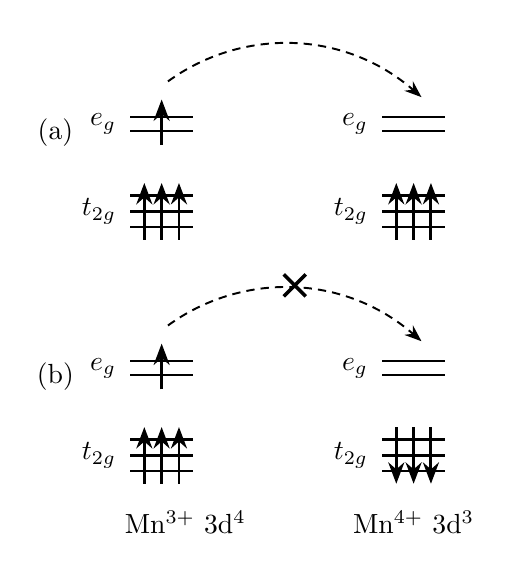
\begin{tikzpicture}[line width=0.8pt,>=Stealth]
\tikzset{lvl/.style={line width=0.9pt},
  up/.style={line width=1.05pt,->},
  dn/.style={line width=1.05pt,->},
  hop/.style={line width=0.7pt,dash pattern=on 3pt off 2.2pt,->}}
% ================= row (a) =================
\node at (-1.35,0.10) {(a)};
% left column e_g (occupied)
\draw[lvl] (-0.4,0.30) -- (0.4,0.30);
\draw[lvl] (-0.4,0.12) -- (0.4,0.12);
\node[left] at (-0.45,0.21) {$e_g$};
\draw[up] (0,-0.06) -- (0,0.52);
% right column e_g (empty)
\draw[lvl] (2.8,0.30) -- (3.6,0.30);
\draw[lvl] (2.8,0.12) -- (3.6,0.12);
\node[left] at (2.75,0.21) {$e_g$};
% t2g left: three up electrons
\foreach \i in {0,1,2}{\draw[lvl] (-0.4,-0.70-0.20*\i) -- (0.4,-0.70-0.20*\i);}
\node[left] at (-0.45,-0.90) {$t_{2g}$};
\foreach \x in {-0.22,0,0.22}{\draw[up] (\x,-1.26) -- (\x,-0.54);}
% t2g right: three up electrons
\foreach \i in {0,1,2}{\draw[lvl] (2.8,-0.70-0.20*\i) -- (3.6,-0.70-0.20*\i);}
\node[left] at (2.75,-0.90) {$t_{2g}$};
\foreach \x in {2.98,3.2,3.42}{\draw[up] (\x,-1.26) -- (\x,-0.54);}
% allowed hop
\draw[hop] (0.08,0.75) .. controls (1.0,1.42) and (2.3,1.42) .. (3.3,0.55);
% ================= row (b) =================
\begin{scope}[shift={(0,-3.1)}]
\node at (-1.35,0.10) {(b)};
% left column e_g (occupied)
\draw[lvl] (-0.4,0.30) -- (0.4,0.30);
\draw[lvl] (-0.4,0.12) -- (0.4,0.12);
\node[left] at (-0.45,0.21) {$e_g$};
\draw[up] (0,-0.06) -- (0,0.52);
% right column e_g (empty)
\draw[lvl] (2.8,0.30) -- (3.6,0.30);
\draw[lvl] (2.8,0.12) -- (3.6,0.12);
\node[left] at (2.75,0.21) {$e_g$};
% t2g left: three up
\foreach \i in {0,1,2}{\draw[lvl] (-0.4,-0.70-0.20*\i) -- (0.4,-0.70-0.20*\i);}
\node[left] at (-0.45,-0.90) {$t_{2g}$};
\foreach \x in {-0.22,0,0.22}{\draw[up] (\x,-1.26) -- (\x,-0.54);}
% t2g right: three DOWN (antiparallel core spins)
\foreach \i in {0,1,2}{\draw[lvl] (2.8,-0.70-0.20*\i) -- (3.6,-0.70-0.20*\i);}
\node[left] at (2.75,-0.90) {$t_{2g}$};
\foreach \x in {2.98,3.2,3.42}{\draw[dn] (\x,-0.54) -- (\x,-1.26);}
% forbidden hop
\draw[hop] (0.08,0.75) .. controls (1.0,1.42) and (2.3,1.42) .. (3.3,0.55);
\draw[line width=1.3pt] (1.55,1.12) -- (1.83,1.40);
\draw[line width=1.3pt] (1.55,1.40) -- (1.83,1.12);
\end{scope}
% ---------- column labels ----------
\node at (0.3,-4.85) {Mn$^{3+}$ 3d$^4$};
\node at (3.2,-4.85) {Mn$^{4+}$ 3d$^3$};
\end{tikzpicture}
\end{document}
